\chapter{Background}
\label{c:Background}

\section{Program Comprehension}

\section{Static vs. Dynamic Analysis}

\section{Object Interaction Modeling}
\subsection{UML Object Diagrams}
\subsection{UML Sequence Diagrams}

\begin{figure}
	\centering
	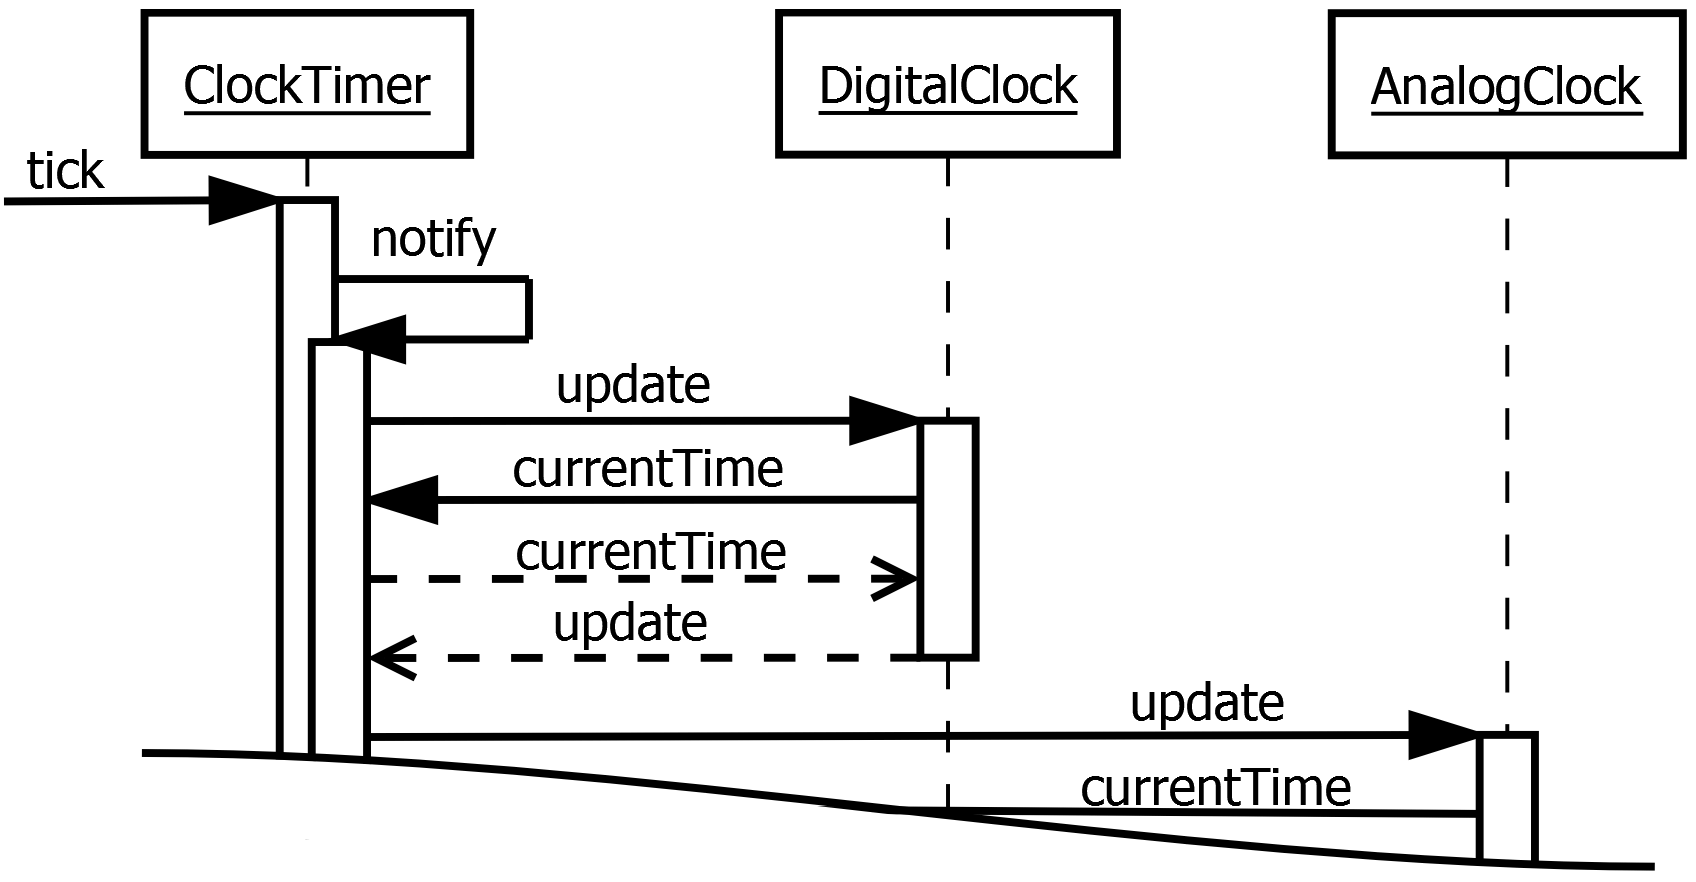
\includegraphics[width=0.6\textwidth]{../images/02-Sequence}
	\caption[TOC Caption]{UML Sequence Diagram}
	\label{fig:ModelingSequence}
\end{figure}


\subsection{UML Communication Diagrams}

\begin{figure}
	\centering
	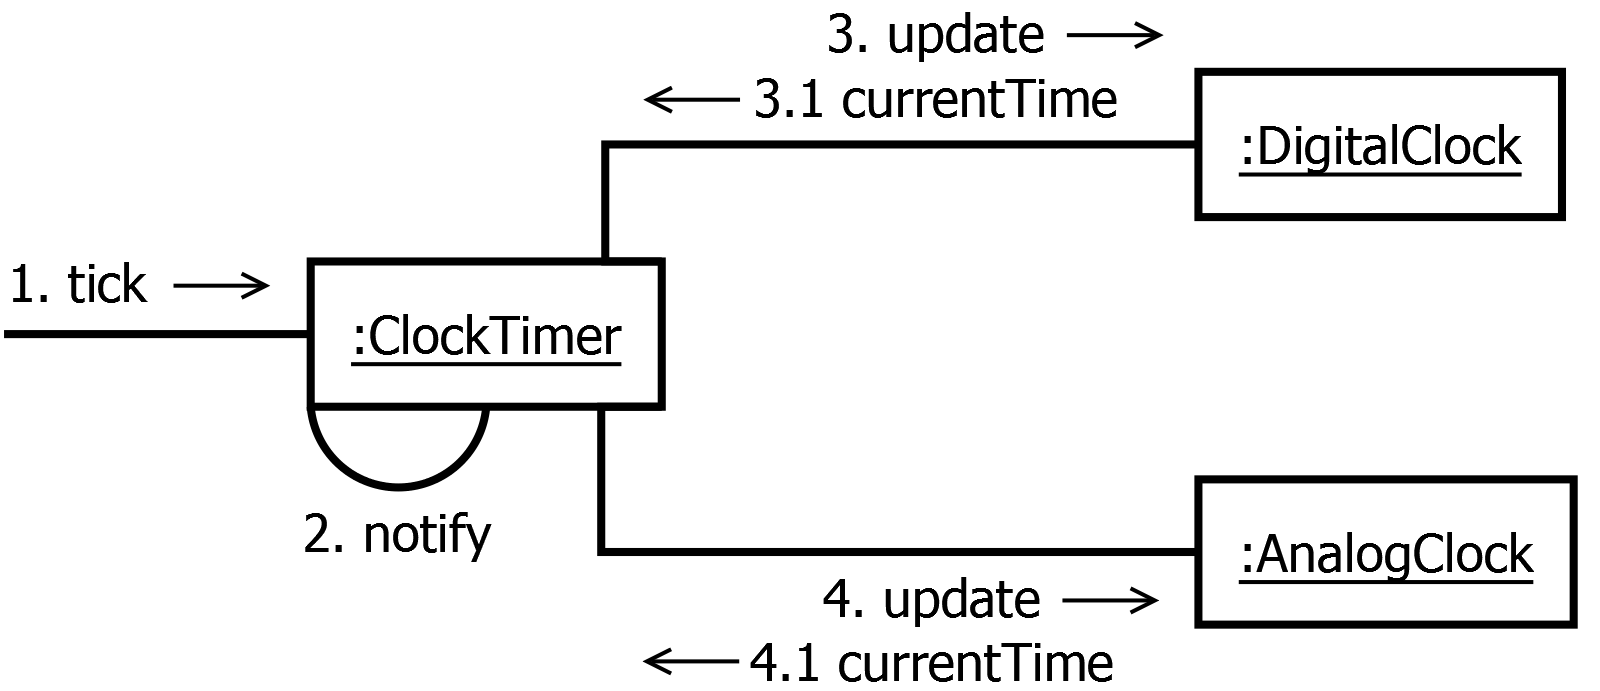
\includegraphics[width=0.6\textwidth]{../images/02-Communication}
	\caption[TOC Caption]{UML Communication Diagram}
	\label{fig:ModelingCommunication}
\end{figure}

\subsection{Discussion}
Due to the fact that the Unified Modeling Language makes a strict distinction between structural and behavioral diagrams, none of them offers a combined view on object interactions as well as the internal state of objects.
However, to understand the behavior of object-oriented systems, it is important to get an insight into both.
Interactions have to be depicted in order to make the behavior of a system perceivable to the observer.
To understand why a systems behaves the way it does, the internal state of objects has to be unveiled.

Apart from this fundamental problem, the diagrams all have drawbacks of their own that make them inadequate for our objectives.

\section{Challenges}